\newpage
\hypertarget{sec:invertCard}{}
\section{Inverting a card}
\genHeader

This next SDM \emph{inverts} a card by swapping its back and face values (Fig.~\ref{fig:goal_invert}). This therefore ``turns a card around'' in the learning
box. This action makes sense if a user wants to try learning, for example, the definition of a word in the other (target) language. Instead of guessing the
definition of every word when presented with the term, perhaps they would like to guess the term when presented with the definition. This method doesn't need to
accept any parameters -- it'll use a bound \texttt{this} object variable.

\vspace{0.5cm}

\begin{figure}[htbp]
	\centering
    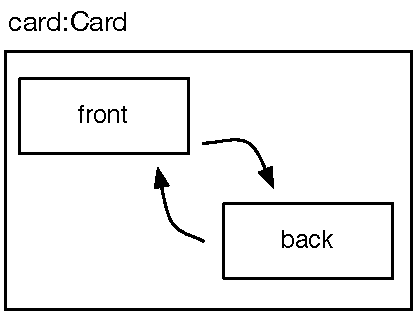
\includegraphics[width=0.4\textwidth]{goal_invert.pdf}
 	\caption{Inverting the attributes of a \texttt{Card}}
 	\label{fig:goal_invert}
\end{figure}
\FloatBarrier

Something new that we'll use in this SDM are \emph{assignments}\define{Assignments} to set the attributes of a \texttt{temp} object variable with \texttt{card},
then again to actually swap the \texttt{card} values. An assignment is simply an attribute constraint\footnote{Which we first encountered in \texttt{check}}
with a \texttt{`:='} operator. Though it may be slightly confusing to refer to an assignment as a constraint, if you think about it, \emph{everything} can be
considered as a constraint that must be fulfilled using different strategies.

With \texttt{invert}, a successful match is achieved not by searching as you would with a comparison (\texttt{==, >, <, \ldots}), but by \emph{performing} the
above assignment. If the assignment cannot be completed, the match is invalid. Similarly, non-context elements (set to create or destroy) can be viewed as
structural constraints that are fulfilled when the corresponding element is created or destroyed.  A constraint is therefore a unifying concept similar to
``everything is an object'' from OO, and ``everything is a model'' from metamodelling.  If you're interested in why \emph{unification} is considered cool, check
out~\cite{BEZ05}.

\newpage
\hypertarget{invertCard vis}{}
\subsection{Implementing invert}
\visHeader

\begin{itemize}

\vspace{0.5cm}

\item[$\blacktriangleright$] If you've completed all the work so far, you've got to be \emph{really} good at SDMs now. Model the simple story diagram
depicted in Fig.~\ref{ea:sdm_invertEmpty}.

\vspace{0.5cm}

\begin{figure}[htbp]
\begin{center}
  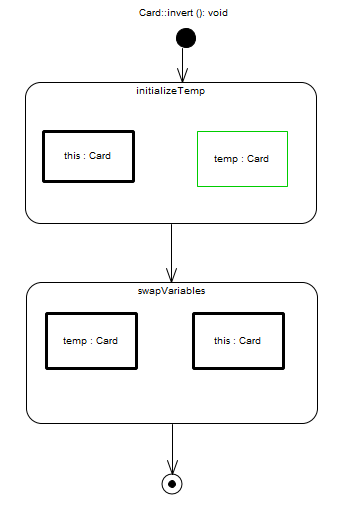
\includegraphics[width=0.6\textwidth]{ea_invertEmpty}
  \caption{Imperative control layer for inverting a card}  
  \label{ea:sdm_invertEmpty}
\end{center}
\end{figure}

\item[$\blacktriangleright$] Note that the binding operator on the first \texttt{temp} object variable is set to \texttt{create} (thus the green
border). This means that we actually \emph{create} a new object, and do not pattern match to an existing one in our model.

\item[$\blacktriangleright$] This activity will need four assignment constraints - two in \texttt{in\-it\-ia\-lize\-Temp} (to store the ``opposite'' values),
and two in \texttt{swapVariables} (to switch the values). Create your first assignment constraint by going to the created \texttt{temp} card and using the
`\texttt{:=}' operator to set the \texttt{temp.back} value to \texttt{this.face} (Fig.~\ref{ea:sdm_invertAssignment}).

\begin{figure}[htbp]
\begin{center}
  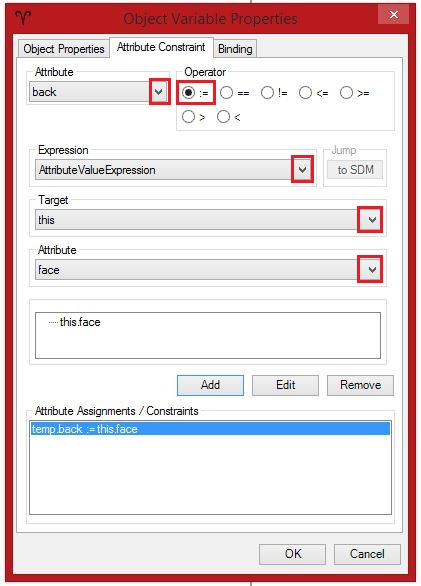
\includegraphics[width=0.7\textwidth]{ea_invertAttConstAssign}
  \caption{Store the \texttt{back} and \texttt{face} values of the card in \texttt{temp}}  
  \label{ea:sdm_invertAssignment}
\end{center}
\end{figure}

\clearpage

\vspace*{0.5cm}

\item[$\blacktriangleright$] Complete the SDM with the remaining constraints according to Fig.~\ref{ea:sdm_invertComplete} below.

\vspace{0.5cm}

\begin{figure}[htbp]
\begin{center}
  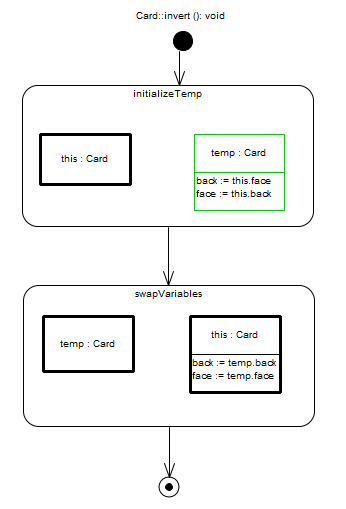
\includegraphics[width=0.7\textwidth]{ea_invertComplete}
  \caption{Swap back and face of the card}  
  \label{ea:sdm_invertComplete}
\end{center}
\end{figure}

\vspace{0.5cm}

\item[$\blacktriangleright$] Believe or not, that's it! Check out how this method is implemented in the textual syntax by reviewing
Fig.~\ref{eclipse:invertPatterns} in the next section. You don't \emph{have} to export and build to Eclipse, but it's always nice to confirm your work is error
free.

\jumpSingle{invert close} 

\end{itemize}


\newpage
\subsubsection{Inversion review}
\genHeader
\hypertarget{invert close}{}

Before we start the next SDM, let's quickly review one point. Have you considered why the \texttt{temp} object variable is bound in the second pattern for
\texttt{invert}, (\texttt{swap variables}), but not where it's first defined in \texttt{initialize temp}?\footnote{See \Cref{ea:sdm_invertComplete}} This is a new case for bound variables that we haven't treated yet!

Until now, we have seen object variables that can be bound to (1) an argument of the method (set when the method is invoked), or (2) the
current object (\texttt{this}) whose method is invoked. In both cases, the object to be matched is completely determined by the context of the method before
the pattern matcher starts. This means that it does not need to be determined or found by the pattern matcher.

Setting \texttt{temp} as bound in \texttt{Swap variables} is a third case in which an object variable is bound to a value determined in a \emph{previous}
activity node without using a special expression type. In this SDM, this means \texttt{temp} will be bound to the value determined for a variable
of the same name in the previous node, \texttt{Initialize temp}. This binding feature enables you to refer to previous matches for object variables in the
preceding control flow.

On a separate note, you're just over halfway through completing this part of the eMoflon handbook, so give your brain a small break. Take a walk, pour
yourself another coffee, and check out one of my favourite jokes:
\syntax{How do you wake up Lady Gaga?}

\vspace{0.5cm}

\syntax{Poke her face!}


